\section{Learning seed costs for a wider set of targets}
\label{sec:family-cost}
The broad test in Section~\ref{sec:extended-coverage} showed that the earlier models often fell back to native choices. We therefore extend cost training to vacuum, two-point, and scattering families, and make the decision before Kira generates equations. The new comparison asks whether a learned choice can improve on a separately tuned fixed choice for each family. Kira's existing seeding and equation selection remain the starting point~\cite{Kira3}, and every selected calculation retains exact algebra and recovery.

\subsection{Training and integration}
Each target batch has either two extra denominator powers or one extra denominator power with one numerator power when an auxiliary coordinate exists. We shift these powers across up to three lines. The training grid contains 22 labelled family-and-loop entries at one through four loops. The family definitions follow Appendices~\ref{app:coverage} and~\ref{app:families}; Appendix~\ref{app:family-cost} specifies the new profiles and target construction. These entries have rational external invariants and symbolic dimension. The two-loop ladder and planar double-box entries share a denominator routing and use different assignments of the external invariants. Thus the entry count does not count distinct graph topologies.

The model predicts the measured cost of ten seed settings, using loop order, denominator structure, target count, powers, and numerator positions. We fit shared decision trees and family-specific one-split cost trees, as well as random forests~\cite{Breiman2001Forest}, and extremely randomized trees~\cite{Geurts2006ExtraTrees}. The training set contains 111 complete cost examples from earlier training records and a new parameter profile. Separate validation selects the tree model, decision margin, and fixed control for each family. We retain a candidate model when it reduces the summed validation time for the two target shapes by at least 3\% relative to that family's best fixed setting. We then confirm each proposed learned gain on profile $h=1113$, using three repetitions. We retain the learned choice only if it again saves at least 3\% in total and neither target shape is more than 3\% slower than its fixed control. These are validation conditions, not guarantees for future targets. The reference coefficients never enter the model.

Kira first attempts the selected seed region. If the calculation does not reduce the targets in the supplied basis, it retries native bounds and then expanded bounds. The cost includes each failed attempt. A small initial region can therefore cost more than a larger region that succeeds immediately. The combined application retains the exact scalar formula when it applies, uses a new family choice only when validation also improves on the previous application, and otherwise keeps the previous application. It preserves the earlier sparse-seed and equation-filter models in their existing domains. The exact scalar check runs before the general native index limit because its formula does not need native sector storage.

\subsection{Reserved tests and attribution}
The reserved grid has 44 batches at a separate parameter profile. It shares graph structures and target patterns with training, while changing kinematic values and, where the target list allows, line positions. 41 batches give matched nontrivial reductions under all five methods. The coverage record contains 3 requests without a checked reference and 0 requests with an application failure. These outcomes remain outside the matched timing ratio. Each matched method runs five times in rotated order. The timer starts with a fresh process and includes imports, model loading, prediction, equation generation, algebra, exact coefficient checks, retries, and process exit. Master discovery and the enlarged independent reference check remain separate. These comparisons test coefficient agreement in the supplied basis; they leave a proof of global basis minimality outside their scope. Each attempt has a 60-second budget, including a ten-second completion reserve; reference attempts have 90 seconds with the same reserve.

The native, fixed, and learned comparisons use the same exact Kira implementation. The native control is the project's preceding exact executable with ML disabled, including its existing exact preparation changes. The native control uses the target-derived bounds, the fixed control uses one validation-selected action per family, and the learned method can change that action from the target features. Their summed per-batch median times are 63.538, 58.707, and 55.886 seconds. Thus the learned-to-native ratio is 0.880, while the isolated learned-to-fixed ratio is 0.952, with paired-repetition interval [0.890, 1.026]. The predictor runs on 2 matched batches and changes the fixed action on 1. The learned-to-fixed ratio over predictor calls is 0.938. Inactive domains use the same action under the fixed and learned labels, so their differences measure run variation. In particular, the nonplanar mixed batch uses identical bounds and equation counts in both conditions. Its timing difference cannot be assigned to ML.

The common master discovery takes 125.450 seconds on the matched requests; the independent enlarged check takes a further 263.492 seconds. Adding discovery to each application gives 184.884 seconds for the previous method and 181.901 seconds for the combined method. The added training and validation cost measurements take 2238.664 seconds, excluding reference construction and model fitting. These offline costs are separate from each production request. The discovery runs also compute the reference reductions, so adding their time to a second application measures this two-stage workflow. The primary speed ratios apply to reductions with a supplied basis.

The previous application takes 59.435 seconds and the combined application takes 56.451 seconds on the same workload. Their ratio is 0.950, with interval [0.877, 0.990]. This comparison measures the whole application change, including fixed choices and exact formula selection. It does not assign the full difference to machine learning. All matched outputs pass 12400 coefficient-pair checks, including repeated measurements.

\begin{table}[!htbp]\centering\small
\caption{Complete time ratios by physical family and loop order. Values below one mean less time. The Changed column counts batches in which the model selects a different seed action from the fixed control. Ratios in inactive domains measure run variation. The first ratio compares the learned and fixed conditions; the second measures the combined application.}
\label{tab:family-cost}
\begin{tabular}{@{}lrrrr@{}}\toprule
Family and loops & Batches & Changed & Learned/fixed & Combined/previous\\\midrule
bubble box L2 & 2 & 0 & 0.991 & 0.743\\
bubble box L3 & 2 & 1 & 0.938 & 0.996\\
double box L2 & 2 & 0 & 1.000 & 1.016\\
ladder L1 & 2 & 0 & 1.022 & 0.963\\
ladder L2 & 2 & 0 & 0.999 & 1.010\\
nonplanar box L2 & 2 & 0 & 0.844 & 0.984\\
one mass box L1 & 2 & 0 & 1.000 & 0.919\\
pentagon L1 & 2 & 0 & 0.974 & 0.936\\
propagator massive L1 & 2 & 0 & 0.999 & 0.973\\
propagator massive L2 & 2 & 0 & 0.991 & 0.928\\
propagator massive L3 & 2 & 0 & 1.013 & 0.741\\
propagator massless L2 & 2 & 0 & 0.996 & 0.954\\
propagator massless L3 & 2 & 0 & 0.930 & 0.950\\
propagator massless L4 & 1 & 0 & 0.999 & 0.980\\
vacuum all mass L1 & 2 & 0 & 1.063 & 0.935\\
vacuum all mass L2 & 2 & 0 & 1.019 & 0.969\\
vacuum all mass L3 & 2 & 0 & 1.013 & 0.878\\
vacuum one mass L1 & 2 & 0 & 1.011 & 0.922\\
vacuum one mass L2 & 2 & 0 & 1.004 & 0.919\\
vacuum one mass L3 & 2 & 0 & 0.996 & 0.946\\
vacuum one mass L4 & 2 & 0 & 0.972 & 0.939\\
\bottomrule\end{tabular}\end{table}
\begin{figure}[!htbp]\centering
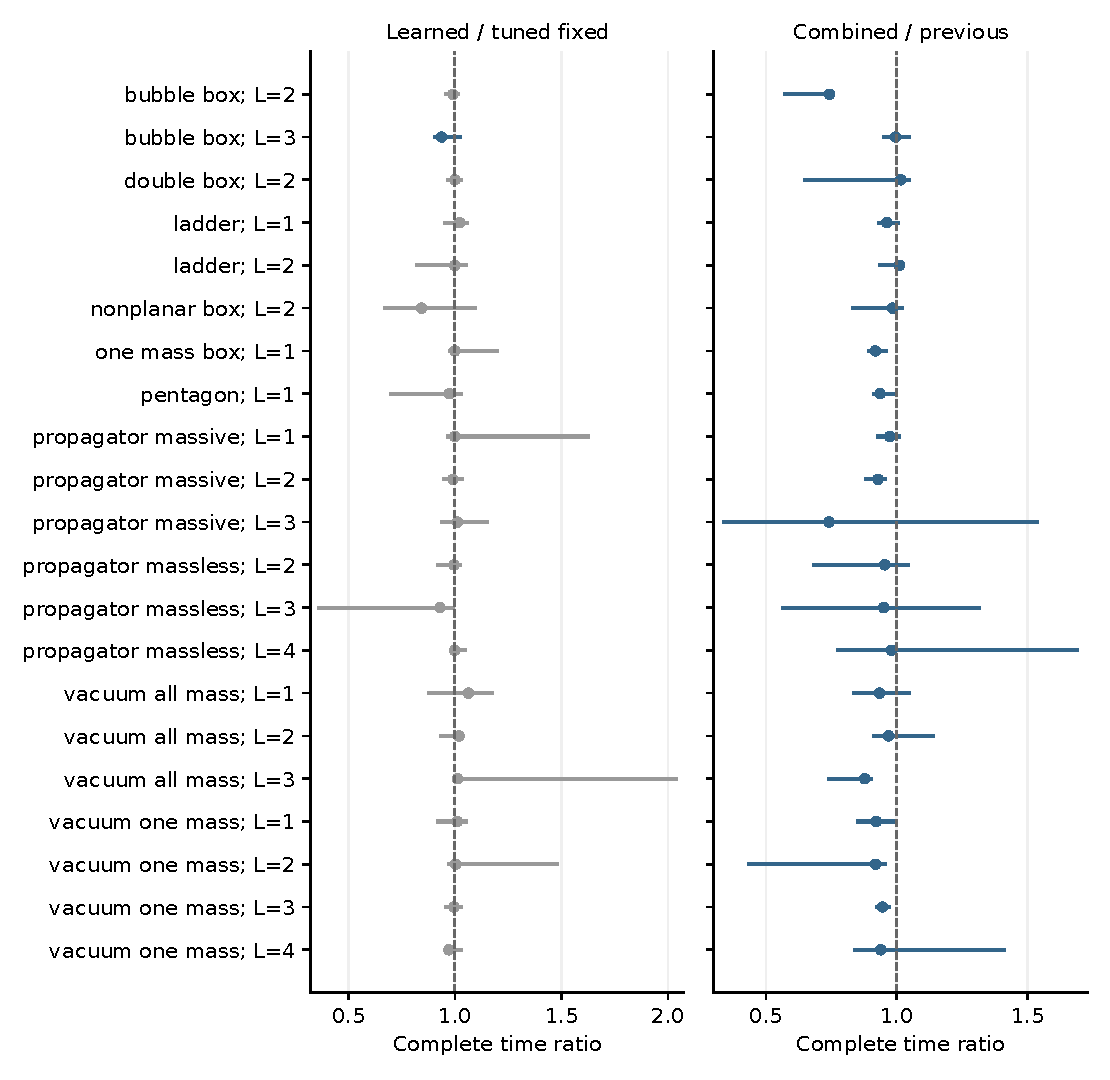
\includegraphics[width=\linewidth]{paper_figures/family_cost.pdf}
\caption{The learned and combined comparisons answer different questions. Points show complete-time ratios, horizontal lines show paired-repetition intervals, and the dashed line marks equal time. Gray points in the left panel have no changed model choice and show timing variation between identical actions. Each interval describes timing variation for the fixed measured workload. It does not describe all possible integrals of that family.}
\label{fig:family-cost}
\end{figure}\FloatBarrier

\subsection{Higher-loop preparation and exact scalar coverage}
The earlier allocation failures occur before a model selects seeds. The tested implementation creates three arrays indexed by sector, whose native size grows as $2^N+1$ for $N$ integral coordinates. Auxiliary numerator coordinates increase $N$ even when they never become denominators in any declared sector. We restrict these arrays and the sector-order table to the already admitted sector domain while keeping every relation and relative ordering in that domain. We also obtain the smallest nontrivial sector size by counting known trivial sectors, which avoids an exhaustive scan. Appendix~\ref{app:family-cost} gives the bound and its conditions. This is an exact storage change, and its gain is separate from the learned-choice comparison above.

The storage test retains 16 predefined requests and their full outcomes: 5 complete comparisons, 1 checked bounded reduction with an incomplete allocation control, 9 incomplete reference calculations, 1 incomplete independent reference check. The new calculation first discovers a basis and then checks it with increased numerator bounds and a different ordering. Where both storage methods complete, three repeated reductions compare coefficients and times in that common basis. A native allocation failure has no finite completion time and therefore supplies no finite speedup ratio. The detailed notes and evidence retain each failed request. A completed 64-bit reference whose enlarged check reaches the initial 60-second budget receives one 180-second check attempt. The increased numerator bound, changed ordering, exact comparison, and memory and storage limits remain unchanged; the initial failure remains in the evidence. Application timing retains its original budget.

A separate scalar test uses the full scalar-product coordinate representation at every loop order from one through twelve. All twelve batches pass the independently implemented raising recurrence of Appendix~\ref{app:extended-coverage}, with three targets per batch. Auxiliary powers remain zero. This extends the admitted representation of the exact scalar formula, including coordinate counts above the native interface limit. It establishes neither general twelve-loop native IBP reduction nor a twelve-loop learned gain.

The measured family ratios determine where the new choices help. Some families retain fixed or previous choices, and some larger calculations remain limited by preparation or algebra. These results do not establish a learned speedup for every integral type or every loop order.
\paragraph{Wider ordering representation.} The separate 128-bit test retains 16 predefined requests: 4 complete comparisons, 9 incomplete reference calculations, 3 incomplete independent reference checks. Both allocation methods use the wider representation. It addresses the ordering-label capacity and leaves coefficient arithmetic unchanged. The native coordinate limit and the cost of preparing IBP polynomials still apply.

\begin{table}[!htbp]\centering\small
\caption{Exact sector-storage checks with a common weight width in each pair. Times are median complete seconds; memory is peak process-tree resident memory in MiB. An incomplete native run has no finite time ratio. Only rows with a checked bounded reduction appear here; all other requests remain in the reported outcome counts.}
\begin{tabular}{@{}lrrrrr@{}}\toprule Family and loops & Bits & Native s & Bounded s & Native MiB & Bounded MiB\\\midrule
ladder L2 & 64 & 6.571 & 6.156 & 57.9 & 64.3\\
propagator massive L2 & 64 & 0.823 & 0.797 & 20.7 & 20.7\\
vacuum all mass L3 & 64 & 1.082 & 1.074 & 21.4 & 21.3\\
vacuum all mass L5 & 64 & incomplete & 45.218 & 142.3 & 168.7\\
vacuum one mass L3 & 64 & 0.742 & 0.737 & 20.0 & 20.2\\
vacuum one mass L5 & 64 & 11.099 & 10.321 & 132.6 & 110.9\\
ladder L2 & 128 & 6.802 & 6.366 & 105.3 & 77.5\\
propagator massive L2 & 128 & 0.795 & 0.785 & 20.9 & 20.8\\
vacuum all mass L3 & 128 & 1.097 & 1.080 & 22.0 & 21.8\\
vacuum one mass L3 & 128 & 0.761 & 0.739 & 20.8 & 20.5\\
\bottomrule\end{tabular}\end{table}\FloatBarrier
The vacuum all mass L5 batch contains 3 targets, including 1 nontrivial reductions in a reference basis of 32 integrals.
The vacuum one mass L5 batch contains 3 targets, including 2 nontrivial reductions in a reference basis of 1 integral.
\subsection{The final combined application}
We then combine the frozen models with an exact route selected from the separate storage validation. Low-loop bounded storage requires a measured gain of at least 3\% before deployment. For higher-loop cases that complete with wider weights, validation chooses the faster complete allocation method. Each selected route must also pass a complete application check. Other inputs keep the previous exact executable. The fitted model parameters remain unchanged. For deployment, the confirmation measurements also distinguish the dotted and mixed target patterns. A pattern uses the new learned choice only if its confirmation median is at least 3\% below both the fixed control and the previous application. This selects the mixed three-loop bubble-box pattern and retains the previous route for its dotted counterpart. We freeze this gate before the final test. A second matched comparison reruns the native control, previous application, fixed choice with validation-selected exact routes, learned choice with validation-selected exact routes, and final combined application. It uses a fresh reserved profile, $h=1151$, with the same graph and target construction and five rotated fresh-process repetitions. Each new request receives an independently discovered and checked master basis. This stage measures the combination directly; it does not multiply gains from separate experiments.

The final grid contains 44 batches, of which 41 give matched nontrivial reductions, 3 lack a checked reference, and 0 have application-failure records. Native and previous application totals are 66.045 and 58.729 seconds. The fixed and learned choices with validation-selected exact routes take 57.067 and 56.576 seconds, while the final combined application takes 56.461 seconds. The isolated learned-to-fixed ratio is 0.991, with interval [0.954, 1.019]. The final-to-previous ratio is 0.961, with interval [0.934, 1.021]. The final-to-native ratio is 0.855.

Bounded storage acts in 4 matched final batches; the other matched batches retain the previous storage route. The common reference construction takes 123.958 seconds and its independent checks take 330.029 seconds. Including reference construction gives 182.687 seconds for the previous two-stage workflow and 180.419 seconds for the final two-stage workflow.

The target-pattern gate activates on 1 matched batch. In this subset, the learned-to-fixed ratio under the same exact route is 0.839, with interval [0.780, 0.841]. The final-to-previous ratio is 0.826. The learned-to-native ratio is 1.006, with interval [0.931, 1.023]. Thus a gain against the tuned fixed control does not establish a gain against native bounds. This small subset measures the new model's deployed domain and does not establish transfer to other graph structures.

The summed median numbers of generated IBP equations in this subset are 26,095 for the fixed control and 19,153 for the learned choice, including recovery attempts. Native bounds generate 19,153 equations. For this mixed target batch, the model selects the native numerator-rank bound with relaxed truncation. This avoids the extra numerator-rank seeds in the family-wide fixed setting. These counts explain equation-generation work and do not count every algebraic operation.

All matched final outputs pass 12475 coefficient-pair checks. This comparison includes both the exact changes and the validation-selected application, while its learned-to-fixed control isolates the model's extra contribution.

\begin{table}[!htbp]\centering\small
\caption{Final combined comparison. Both learned and fixed controls use the same validation-selected exact route. The final application also retains exact scalar formulae and validated previous choices. The Changed column counts model decisions that differ from the fixed action.}
\label{tab:family-combined}
\begin{tabular}{@{}lrrrr@{}}\toprule
Family and loops & Batches & Changed & Learned/fixed & Final/previous\\\midrule
bubble box L2 & 2 & 0 & 1.179 & 0.613\\
bubble box L3 & 2 & 1 & 0.929 & 0.922\\
double box L2 & 2 & 0 & 1.025 & 0.981\\
ladder L1 & 2 & 0 & 1.029 & 0.871\\
ladder L2 & 2 & 0 & 1.043 & 1.068\\
nonplanar box L2 & 2 & 0 & 0.981 & 0.988\\
one mass box L1 & 2 & 0 & 1.017 & 1.010\\
pentagon L1 & 2 & 0 & 1.127 & 0.945\\
propagator massive L1 & 2 & 0 & 1.104 & 1.115\\
propagator massive L2 & 2 & 0 & 1.104 & 0.986\\
propagator massive L3 & 2 & 0 & 0.951 & 0.767\\
propagator massless L2 & 2 & 0 & 1.042 & 0.989\\
propagator massless L3 & 2 & 0 & 0.893 & 1.065\\
propagator massless L4 & 1 & 0 & 0.857 & 1.215\\
vacuum all mass L1 & 2 & 0 & 0.901 & 0.906\\
vacuum all mass L2 & 2 & 0 & 1.026 & 1.192\\
vacuum all mass L3 & 2 & 0 & 0.825 & 0.965\\
vacuum one mass L1 & 2 & 0 & 0.928 & 0.941\\
vacuum one mass L2 & 2 & 0 & 1.010 & 0.996\\
vacuum one mass L3 & 2 & 0 & 1.003 & 0.853\\
vacuum one mass L4 & 2 & 0 & 0.968 & 0.966\\
\bottomrule\end{tabular}\end{table}
\begin{figure}[!htbp]\centering
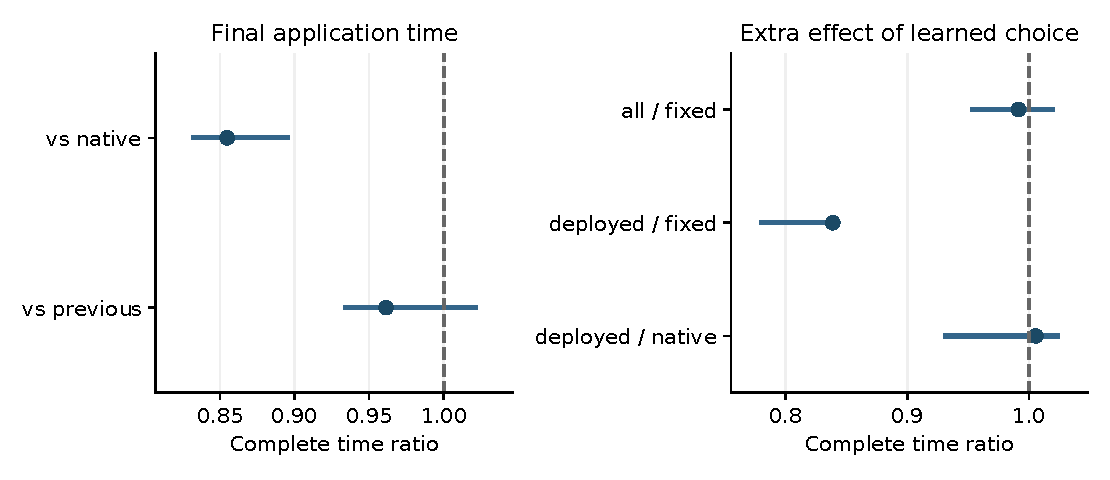
\includegraphics[width=\linewidth]{paper_figures/family_combined.pdf}
\caption{The final comparison separates complete application time from the extra effect of learned seed choices. The right panel compares the learned choice with fixed and native controls under the same exact route. The deployed subset contains the target pattern selected before testing, on which the model changes the seed action. Inactive domains use identical actions and contribute run variation to the all-matched comparison. Points show ratios and lines show paired-repetition intervals; the two horizontal scales resolve their different magnitudes.}
\label{fig:family-combined}
\end{figure}\FloatBarrier
